\chapter{Il progetto di \textit{stage}}

\section{Il rapporto dell'azienda con gli \textit{stage} universitari}
\label{sec:rapporto-eggon-stage}

% Descrizione di come \textit{Eggon} integra gli stagisti universitari all'interno del proprio processo produttivo, affidando loro attività concrete e direttamente collegate allo sviluppo dei prodotti aziendali, anziché incarichi marginali o puramente formativi. Tale approccio riflette la visione dell'innovazione descritta nella Sezione~\ref{sec:propensione-innovazione}. Lo \textit{stage} viene quindi inquadrato come parte di una strategia più ampia, nella quale il coinvolgimento degli stagisti rappresenta un canale ricorrente per affrontare attività di espansione e di \textit{porting} che, diversamente, richiederebbero l'impiego di risorse interne dedicate.

Eggon non concepisce gli \textit{stage} come semplici esercitazioni didattiche o attività marginali. Al contrario, integra gli stagisti come parte attiva del processo produttivo, affidando loro attività direttamente collegate allo sviluppo e alla manutenzione dei prodotti aziendali.

Durante le mie 8 settimane previste dall'università, Eggon accoglieva contemporaneamente cinque stagisti, suddivisi su tre progetti distinti, ciascuno con obiettivi e tecnologie diverse. Oltre a me, altri tre stagisti hanno iniziato nello stesso periodo: due lavoravano su un progetto di raccolta dati tramite \textit{ESP32}, un \textit{microcontroller} a basso consumo, per il monitoraggio durante l'utilizzo della moto, e uno era impegnato nello sviluppo e manutenzione di NEXUM, il \textit{software} proprietario di Eggon utilizzato per la gestione delle presenze lavorative e della pianificazione dei progetti.

Due settimane dopo l'inizio del mio \textit{stage}, un quinto stagista si è unito a me nel progetto LITD, permettendo una specializzazione dei compiti entro lo stesso ambito di sviluppo videoludico. Successivamente, Eggon ha assegnato un ulteriore stagista al progetto NEXUM, estendendo il supporto su quel fronte.

Questa struttura di distribuzione degli stagisti rivela come Eggon gestisce strategicamente le risorse umane esterne. Piuttosto che concentrare stagisti su un unico progetto, l'azienda li impiega come risposta a esigenze produttive parallele e specializzate. Ogni progetto aveva un \textit{tutor} dedicato, indipendentemente che il gruppo di lavoro fosse costituito da una sola persona o da più stagisti. Questo significa che io e il mio collega stagista condividevamo il medesimo \textit{tutor} e gli stessi obiettivi sul progetto LITD, ma ricevevamo supervisione diretta e costante. Il \textit{tutor} non era una figura generica, ma un membro del \textit{team} Eggon con responsabilità concrete sul progetto stesso, garantendo continuità di conoscenza e allineamento con gli obiettivi aziendali.

Questa configurazione dimostra che gli \textit{stage} non rappresentano per Eggon un canale occasionale o sperimentale, ma piuttosto un meccanismo consolidato e strutturato per esplorare soluzioni su più fronti contemporaneamente. Nel caso di LITD, il progetto era parte di un piano più ampio di estensione del gioco a nuove piattaforme (in particolare Nintendo Switch), un'attività che l'azienda aveva rimandato più volte a causa di priorità organizzative diverse. Affidare questo progetto a degli stagisti ha permesso a Eggon di allocare il \textit{team} interno a compiti che richiedevano una continuità di conoscenza più profonda, mentre gli stagisti (sia singoli che in coppia) acquisivano esperienza in un con\textit{test}o reale di sviluppo su progetti tecnicamente rilevanti. Lo stesso vale per il progetto ESP32, dove l'innovazione tecnologica richiesta beneficiava dell'approccio fresco degli stagisti; e per NEXUM, dove lo sviluppo del \textit{software} interno rappresenta un'infrastruttura critica per l'operatività dell'azienda.

Questo approccio riflette direttamente la visione dell'innovazione che Eggon porta avanti, descritta nella Sezione~\ref{sec:propensione-innovazione}: l'azienda investe in nuove tecnologie e piattaforme, e utilizza gli \textit{stage} come meccanismo organizzato e ricorrente per esplorare soluzioni senza gravare completamente sulle risorse interne. Gli stagisti non sono semplici "aiutanti" di progetto, ma co-protagonisti della strategia di innovazione dell'azienda, un contesto che li accoglie per un periodo temporaneo, ma valorizza i loro contributi integrandoli come parte del prodotto e della strategia aziendale.

\section{Il prodotto: \textit{Lost in the Dungeon}}
\label{sec:prodotto-litd}

% Presentazione del videogioco oggetto dello \textit{stage}, \textit{Lost in the Dungeon}: genere (\textit{card game} con ambientazione \textit{dungeon fantasy}), piattaforme di destinazione, principali meccaniche di gioco dal punto di vista dell'utente finale e stato del progetto al momento dell'avvio dello \textit{stage}. Questa sezione fornisce il con\textit{test}o applicativo necessario per comprendere le scelte progettuali e gli interventi descritti nel Capitolo~3.
 
\textit{Lost in the Dungeon} (di seguito \textit{LITD}) è un videogioco appartenente ai generi \textit{dungeon crawler} e \textit{card game}, sviluppato e distribuito da Eggon a partire dal 2018 su \textit{PC} e su cellulari. Il gioco è disponibile esclusivamente in lingua inglese: per coerenza, in questo documento riporterò i nomi delle sue scene e componenti principali nella lingua originale.
 
Poco dopo il lancio, Eggon ha rimosso la versione \textit{mobile} dal \textit{Google Play Store}, a seguito di un cambiamento nelle \textit{policy} della piattaforma relative alla tipologia di \textit{asset} supportati. Da allora LITD prosegue esclusivamente su \textit{PC}, distribuito tramite Steam.
 
Il gioco si articola in cinque macroscene, collegate tra loro attraverso una schermata centrale che funge da \textit{hub}:
 
\begin{itemize}
    \item \textit{Authentication}, per la selezione o la creazione di uno dei tre \textit{slot} di salvataggio;
    \item \textit{Inn}, lo \textit{hub} che collega tutte le altre scene e ospita anche il \textit{tutorial} e i crediti del gioco;
    \item \textit{Deck Builder}, per la composizione del mazzo di carte con cui affrontare il \textit{dungeon};
    \item \textit{Inventory \& Shop}, per la gestione e l'acquisto degli artefatti che modificano le statistiche del personaggio;
    \item \textit{Dungeons}, articolata a sua volta in due scene (\textit{Dungeon Choose} e \textit{Dungeon Game}), dedicate rispettivamente alla selezione del \textit{dungeon} e allo svolgimento del combattimento vero e proprio.
\end{itemize}
 
La Figura~\ref{fig:section_one} mostra le prime tre scene elencate, mentre la Figura~\ref{fig:section_two} mostra le restanti due: insieme, offrono un riferimento visivo dell'interfaccia con cui il giocatore interagisce in ciascuna scena, utile per comprendere i vincoli di navigazione discussi più avanti in questa sezione.
 
\begin{figure}[H]
    \centering
    \makebox[\textwidth][c]{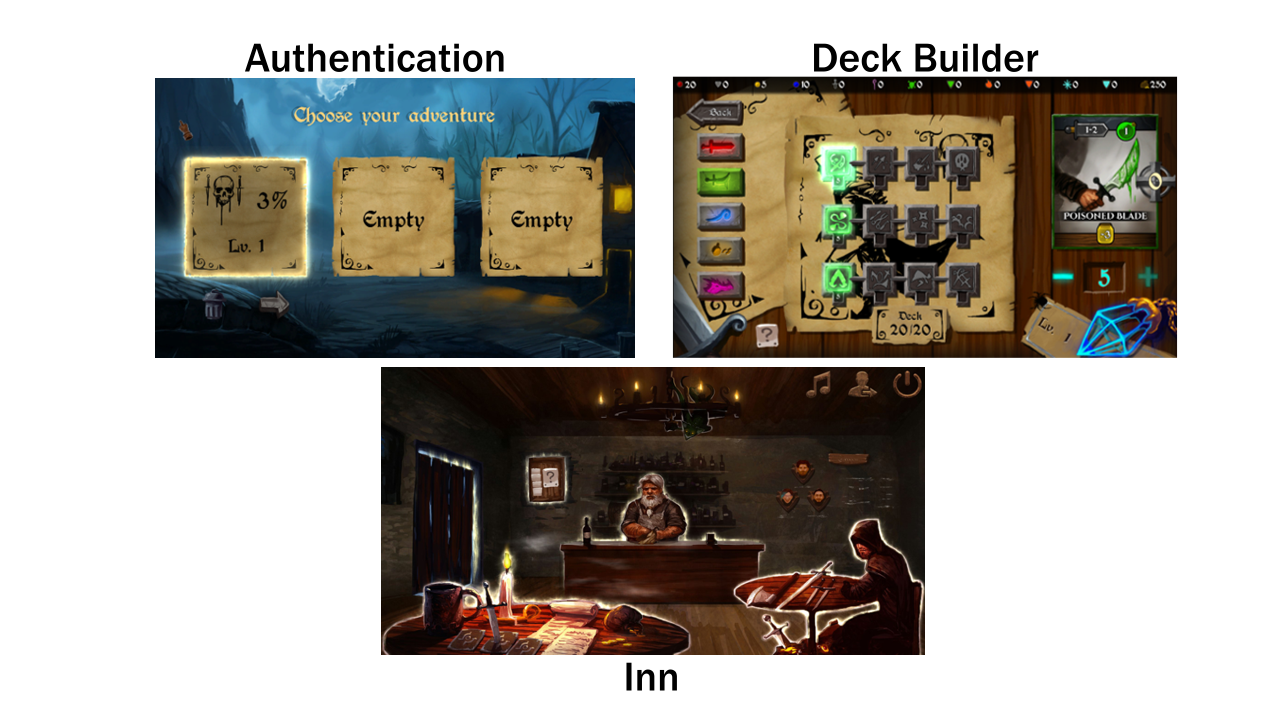
\includegraphics[width=1.15\textwidth]{img/section_one.png}}
    \caption{Schermate di \textit{Authentication}, \textit{Inn} e \textit{Deck Builder}}
    \vspace{0.1cm}
    {\footnotesize Fonte: pagina Steam del prodotto e \textit{screenshot} del gioco\par}
    \label{fig:section_one}
\end{figure}
 
\begin{figure}[H]
    \centering
    \makebox[\textwidth][c]{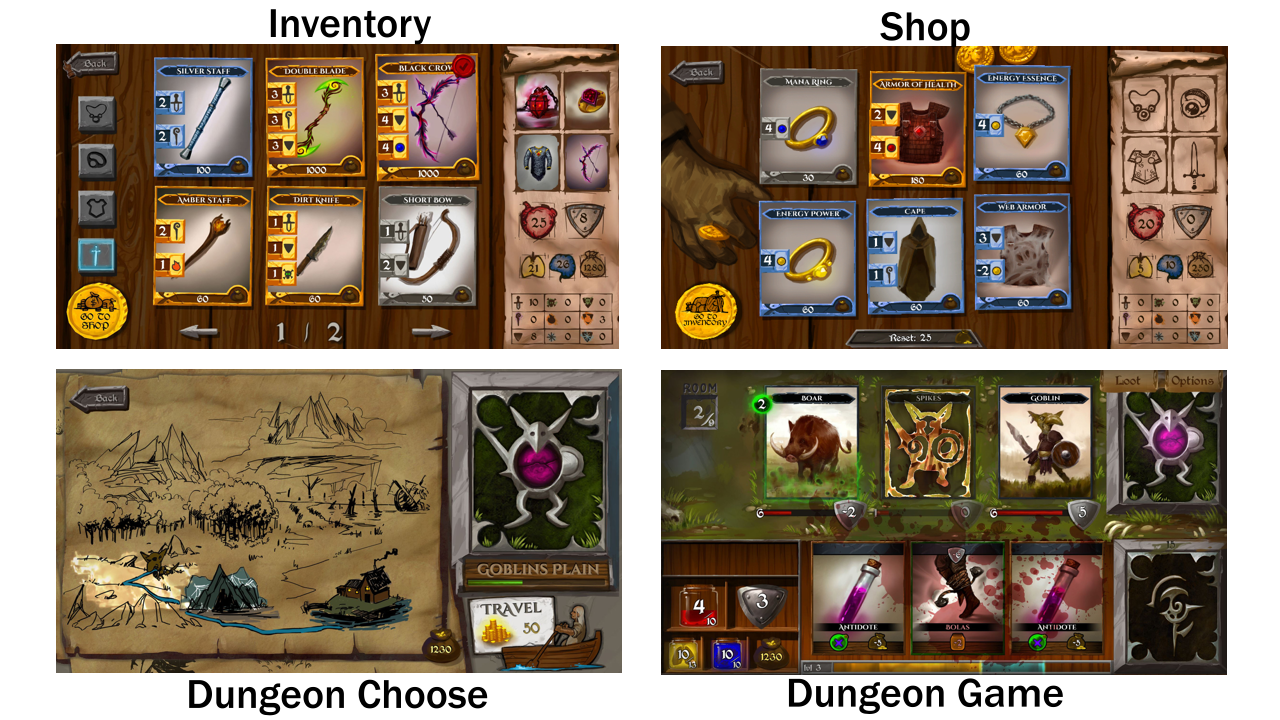
\includegraphics[width=1.15\textwidth]{img/section_two.png}}
    \caption{Schermate di \textit{Inventory \& Shop}, \textit{Dungeon Choose} e \textit{Dungeon Game}}
    \vspace{0.1cm}
    {\footnotesize Fonte: pagina Steam del prodotto e \textit{screenshot} del gioco\par}
    \label{fig:section_two}
\end{figure}
 
Al momento dell'avvio dello \textit{stage}, tutte le scene di LITD condividevano un limite strutturale comune: l'interazione con il gioco richiedeva esclusivamente il \textit{click} del \textit{mouse} su \textit{PC} o al \textit{tap} sull'applicazione \textit{mobile}, senza alcun sistema di navigazione alternativo. Nessuna interfaccia permetteva di selezionari elementi tramite i pulsanti direzionali o dorsali tipici di un \textit{controller}. Questo limite rendeva il gioco, nella sua forma originale, incompatibile con il mercato delle \textit{console}, dove il \textit{platform holder} impone il requisito del supporto per l'\textit{input} da \textit{controller}.
 
A questo problema se ne affiancava un secondo, di natura più circoscritta ma comunque rilevante: le scene \textit{Dungeon Choose} e \textit{Dungeon Game} comunicano con Steam per il tracciamento degli \textit{achievement} di gioco, ma lo strumento di integrazione utilizzato durante lo sviluppo non era più valido al momento dello \textit{stage}, interrompendo di fatto questa comunicazione.
 
L'assenza di supporto per il \textit{controller}, l'integrazione con Steam da ripristinare e il debito tecnico accumulato da un \textit{engine} ormai datato (Unity 2017) costituiscono, nel loro insieme, i problemi concreti che Eggon ha affidato allo \textit{stage}.
%Gli obiettivi discussi in §2.3 rappresentano la declinazione operativa di questi problemi.
 
\section{Obiettivi e vincoli dello \textit{stage}}
\label{sec:obiettivi}

% Descrizione degli obiettivi individuati dall'organizzazione ospitante: realizzazione di un sistema di navigazione completo tramite \textit{controller} in tutte le scene di gioco, attività di \textit{porting} e superamento dei requisiti di certificazione per \textit{Nintendo Switch}, oltre alla risoluzione delle regressioni introdotte dall'aggiornamento del progetto a \textit{Unity 6}. Verranno inoltre illustrati i principali vincoli operativi che hanno caratterizzato il progetto: durata complessiva di otto settimane, necessità di mantenere la piena compatibilità con la \textit{codebase} esistente e svolgimento delle attività in collaborazione con un secondo stagista, mediante una suddivisione degli ambiti di lavoro.

\subsection{Obiettivi iniziali: migrazione dell'\textit{engine}}
\label{sec:obiettivi-migrazione-engine}

Il piano di lavoro iniziale, che ho concordato con Eggon anticipatamente allo \textit{stage}, assegnava una priorità maggiore alla migrazione tecnologica del progetto.
Pianificammo questi obiettivi per portarli a termine rapidamente, lasciando margine di tempo per gli obiettivi successivi discussi in \ref{sec:obiettivi-controller-certificazione}: il \textit{porting} su Nintendo Switch, l'attività più complessa e a maggior rischio dell'intero \textit{stage}.

\begin{table}[h]
\centering
\begin{tabular}{|p{4.5cm}|p{6.5cm}|}
\hline
\textbf{Obiettivo} & \textbf{Metrica di successo} \\
\hline
Migrazione Unity 2017 $\rightarrow$ Unity 6 & 0 errori di compilazione; \textit{warning} ridotti al minimo \\
\hline
Stabilizzazione \textit{build} & \textit{Build} eseguibili su \textit{PC}, iOS e Android, senza \textit{crash} durante la compilazione \\
\hline
Eliminazione \gls{obb} \textit{mobile} & Rimozione completa dell'apparato \textit{OBB} dalla configurazione \textit{mobile} \\
\hline
Compatibilità Steam & Nessun errore di \textit{runtime} specifico della piattaforma Steam \\
\hline
\end{tabular}
\caption{Obiettivi di migrazione, con relative metriche di successo}
\label{tab:obiettivi_migrazione}
\end{table}

A questi obiettivi (si veda \ref{tab:obiettivi_migrazione}) si affiancava un vincolo implicito di compatibilità retroattiva: nessuna modifica introdotta durante la migrazione poteva compromettere i salvataggi o le funzionalità già presenti su \textit{PC} e \textit{mobile}.

Ho affrontato questi obiettivi da solo durante le prime due settimane di \textit{stage}. Nelle settimane successive ho dedicato tempo al consolidamento e alla rifinitura degli stessi obiettivi, con un ritmo più disteso, mentre definivo gli obiettivi successivi del progetto assieme al \textit{tutor}.

\subsection{Obiettivi successivi: navigazione da \textit{controller} e certificazione Nintendo Switch}
\label{sec:obiettivi-controller-certificazione}

Alla terza settimana di \textit{stage} si è unito infatti al progetto LITD il mio collega stagista. Da quel momento abbiamo lavorato insieme sui due obiettivi più critici dell'intero \textit{stage}: entrambi sono emersi dalla consultazione con il \textit{tutor} aziendale, una volta valutato il margine di tempo ottenuto grazie al rapido progresso degli obiettivi iniziali di migrazione (\ref{sec:obiettivi-migrazione-engine}).

\begin{table}[h]
\centering
\begin{tabular}{|p{4.5cm}|p{6.5cm}|}
\hline
\textbf{Obiettivo} & \textbf{Metrica di successo} \\
\hline
Navigazione \textit{controller} & 6/6 scene navigabili esclusivamente tramite \textit{controller} standard \\
\hline
Certificazione Nintendo Switch & 6/6 \textit{test} obbligatori del \textit{Dev Kit} superati \\
\hline
\end{tabular}
\caption{Obiettivi di \textit{porting} verso Nintendo Switch, con relative metriche di successo}
\label{tab:obiettivi_switch}
\end{table}

A questi due obiettivi si affiancava l'implementazione di un sistema di salvataggio conforme al \textit{file system} di Nintendo Switch, basato su \textit{user account} e archivio locale della \textit{console}: condizione necessaria per superare i \textit{test} di certificazione elencati in Tabella~\ref{tab:obiettivi_switch}.

\subsection{Vincoli operativi}
 
Lo svolgimento dello \textit{stage} era vincolato da tre fattori principali:
 
\begin{itemize}
\item durata complessiva di 8 settimane, che l'università impone come vincolo non modificabile;
\item compatibilità retroattiva con la \textit{codebase} esistente durante tutto il lavoro di migrazione (\ref{sec:obiettivi-migrazione-engine}), poiché nessuna modifica poteva compromettere i salvataggi o le funzionalità già distribuite;
\item coordinamento con un secondo stagista sulla medesima \textit{codebase} a partire dalla terza settimana, che richiedeva una suddivisione chiara dei compiti tra navigazione \textit{controller} e certificazione Switch, per evitare conflitti di lavoro sugli stessi \textit{file}.
\end{itemize}
 
La sequenza dei due gruppi di obiettivi descritti in \ref{sec:obiettivi-migrazione-engine} e \ref{sec:obiettivi-controller-certificazione} non era casuale, ma rifletteva una scelta di gestione del rischio entro questi vincoli: completare rapidamente la migrazione, a minore incertezza tecnica, permetteva di destinare la maggior parte delle 8 settimane disponibili alla certificazione Nintendo Switch, l'obiettivo a maggiore rischio per via dei vincoli imposti dal \textit{platform holder} e non pienamente sotto il controllo del \textit{team}. L'arrivo del secondo stagista alla terza settimana, in coincidenza con il completamento degli obiettivi di migrazione, ha permesso di affrontare in coppia il lavoro più oneroso: l'implementazione della navigazione da \textit{controller} su 6 scene e il superamento dei 6 \textit{test} di certificazione, entrambi condizioni necessarie per la pubblicazione su Nintendo Switch.
 
Questa gestione sequenziale, vincolata da un tempo fisso di 8 settimane, riflette lo stesso approccio all'innovazione descritto in \ref{sec:rapporto-eggon-stage}: Eggon delega agli stagisti l'esplorazione tecnica di un nuovo mercato (qui, Nintendo Switch), riservando al \textit{team} interno la sola supervisione tramite il \textit{tutor}, senza investire risorse dedicate a tempo pieno sul progetto durante questo periodo esplorativo.


\section{Motivazioni nella scelta dello \textit{stage}}

%Esposizione delle motivazioni personali che hanno portato a preferire questa opportunità rispetto ad altre proposte disponibili. In particolare, l'interesse per lo sviluppo videoludico e per \textit{Unity} come strumento professionale e la possibilità di lavorare su un prodotto reale destinato a più piattaforme commerciali e l'opportunità di approfondire aspetti tecnici quali la gestione dell'\textit{input} da \textit{controller}, il processo di certificazione per \textit{console}, difficilmente riproducibili in un con\textit{test}o esclusivamente accademico.

L'interesse per il settore videoludico rappresenta una motivazione di lungo termine che ha guidato la mia scelta di studiare informatica. Sin dai primi anni di università, ho considerato il \textit{game development} come un ambito dove il contributo tecnico e creativo convergono in modo significativo, e dove i problemi informatici da risolvere spaziano dalla grafica al \textit{networking}, dall'ottimizzazione delle \textit{performance} alla gestione di sistemi complessi. Questa prospettiva ha influenzato la selezione dei corsi durante il percorso di studi, privilegiando insegnamenti con applicazioni pratiche nel settore.

Tra le proposte di \textit{stage} disponibili, l'opportunità presso Eggon su LITD si è subito distinta per allineamento con questa visione di lungo termine. A differenza di altre fferte circoscritte a progetti di \textit{software business} (gestionali \textit{web}, sistemi informativi aziendali), lo \textit{stage} su LITD rappresentava l'occasione di ontribuire a un prodotto reale destinato al mercato commerciale, sviluppato con una tecnologia professionale quale Unity, ampiamente adottata nell'industria videoludica internazionale. Questo aspetto è stato determinante: non si trattava di un esercizio didattico, ma di un lavoro concreto su un prodotto con una storia, un utenza, e una distribuzione su più piattaforme.

In particolare, lo \textit{stage} prometteva di affrontare sfide tecniche ed ecosistemiche altrimenti inaccessibili. Il \textit{porting} di LITD verso Nintendo Switch richiedeva di approfondire la gestione degli \textit{input} da \textit{controller}, un aspetto centrale dell'esperienza interattiva che raramente emerge nei progetti personali e indipendenti. Il processo di certificazione per \textit{console} rappresenta un elemento ancora più critico: i mondi delle \textit{console} (Nintendo, Sony, Microsoft) sono ecosistemi chiusi e fortemente controllati, dove i produttori regolano rigidamente gli accessi e non disponibili a sviluppatori indipendenti al di fuori di percorsi ufficiali e strutturati. Conoscere come navigare i requisiti di un \textit{platform holder} (in questo caso Nintendo) e implementare soluzioni che li rispettino costituisce un bagaglio di competenze che il mercato del lavoro videoludico ricerca fortemente, ma praticamente inaccessibile al di fuori di con\textit{test}i professionali.

La possibilità di lavorare su un prodotto multi-piattaforma (\textit{PC}, \textit{mobile}, \textit{console}) infine rappresentava un'occasione per toccare con mano le differenze progettuali e tecnologiche che caratterizzano diversi ecosistemi, e come uno studio di gioco professionale naviga tra vincoli e opportunità eterogenei. Questo accresce significativamente il valore formativo dello \textit{stage} rispetto a alternative che avrebbero riguardato sviluppo \textit{software} più generico.

Nel complesso, lo \textit{stage} presso Eggon combinava due esigenze convergenti: la possibilità di specializzarsi nel settore che intendo perseguire professionalmente, e l'accesso a una complessità tecnica e organizzativa che ho ritenuto cruciale per sviluppare competenze spendibili e diversificate nel mercato del lavoro videoludico.

Questa motivazione personale si è tradotta, fin dall'inizio dello \textit{stage}, in obiettivi di apprendimento espliciti, misurabili sulle stesse metriche degli obiettivi aziendali discussi in \ref{sec:obiettivi}, per poterne valutare i risultati nel Capitolo~4 su dati oggettivi piuttosto che su impressioni soggettive. La Tabella~\ref{tab:obiettivi_personali} riassume questi obiettivi personali e il relativo collegamento agli obiettivi aziendali corrispondenti.

\begin{table}[h]
\centering
\begin{tabular}{|p{5cm}|p{6cm}|}
\hline
\textbf{Obiettivo personale} & \textbf{Collegamento alla metrica aziendale} \\
\hline
Acquisire competenza sulla gestione dell'\textit{input} da \textit{controller} & Navigazione \textit{controller} (Tabella~\ref{tab:obiettivi_switch}) \\
\hline
Comprendere il processo di certificazione per \textit{console} & Certificazione Nintendo Switch (Tabella~\ref{tab:obiettivi_switch}) \\
\hline
Gestire la migrazione di una \textit{codebase} esistente & Migrazione Unity 6 (Tabella~\ref{tab:obiettivi_migrazione}) \\
\hline
\end{tabular}
\caption{Obiettivi personali dello stagista, collegati alle metriche aziendali}
\label{tab:obiettivi_personali}
\end{table}